\section{基于P2P网络的信息自主流动机制的方案概述}
本章将阐述基于P2P网络的信息自主流动机制的基本方案。在整套机制中,需要涉及三大研究模块:在文本信息分析与建模的研究中,主要针对互联网中纯文本的信息的非结构化问题,通过数据挖掘和机器学习等方法从中抽取出一部分能够充分表示原文本的特征,并且提出一套适用于各种类型文本的描述方式;在用户兴趣表示与匹配的研究中,主要结合文本信息与用户反馈提出一种具有代表性的兴趣构建方法,从而可以进行用户与用户、用户与资源之间的兴趣相似度计算。在P2P网络路由与发现的研究中,主要利用上述提出的针对资源和用户兴趣的模型,以现在网络为底层架构,构建一层用户兴趣覆盖网络,并提出了网络构建、动态更新与搜索发现等基本方法。最后,基于上述三个模块,本文还设计并实现了一个简易实现的原型系统,主要包括架构设计和功能设计,以此来说明信息自主流动机制的可行性和实际应用价值。

\subsection{文本信息分析与建模}
按照互联网资源的类型可以分为:文本、图片、音乐、视频等。虽然如今涌现了越来越多的诸如音频和视频的流媒体资源,但是互联网上的资源大多任然以文本形式存在,或者可以用文本来代替原有的非文本资源。不仅限于传统的新闻、博客是文本信息,连图片也可以用很成熟的技术来转换成文本,比如百度识图\footnote{http://stu.baidu.com/}就可以自动识别出图片中的物体,即使是视频资源也可以用元信息、标题、评论和弹幕等文本信息进行概括。因此下文主要针对互联网文本信息进行深入研究,并假设其他类型的资源均可以通过已有成熟的方法转换成文本信息。这一小节将根据互联网上四种不同类型的文本,分别提出文本挖掘与建模的方法。

普通的新闻、博客等文章都归类为长文本信息,这类资源一般都是纯文本数据,因此具有两个明显的特征:稀疏性和高维度。举个例子来说:假设给定一由$|\mathcal{V}|$个不同词汇组成的字典$\mathcal{V}$,在由$M$篇文章组成的语料库中,每篇文章$d$的用词都属于词典$\mathcal{V}$,且每篇文章的单词数量不少于$n (0<n\ll W)$。如果直接简单地将文档表示成关于词汇的向量,向量中的每个值表示该词汇在文中的词频,如果该词汇没有在文中出现,则向量中对应的值为0。那么有两点是显而易见的:a)文档向量的维度为$|\mathcal{V}|$,在正常情况下,$|\mathcal{V}|$可以达到百万数量级($10^6$);b)文档向量中最多只有$n$个值大于0,一般情况下,$n$只有几百数量级($10^2$)。这就是纯文本的高维度和稀疏性带来的问题。为了解决这个问题,本文采用基于概率图的主题模型来进行分析,这里先形式化地定义几个重要的基本概念。

对于包含$M$篇文档$d$的语料库$\mathcal{D}$,有$\mathcal{D}=\{d_1,d_2,...,d_M\}$。词汇表$\mathcal{V}$中包含了$W$个不同的词汇$v$。对于文档$d_i$,其中每个单词$w$都取自于$\mathcal{V}$,并且单词可以重复,即$w_i=w_j=v~~(i\ne j, v\in \mathcal{V})$。那么,对于长度为$N$的文档$d$表示为关于单词的向量,$d=\vec{w}=(w_1,w_2,...,w_N)$。

为了简化模型,一般认为文档单词之间是没有先后关系的,换句话说,每个单词相互独立,一个单词出现的概率不会收到另一个单词的影响。因此可以计算文档$d$的生成概率$p(d)$:
\begin{equation}
  p(d)=p(\vec{w})=p(w_1,w_2,...,w_N)=p(w_1)p(w_2)...p(w_N)
\end{equation}
而对于语料库$\mathcal{D}$的生成概率$p(\mathcal{D})$为:
\begin{equation}
  p(\mathcal{D})=p(d_1)p(d_2)...p(d_M)=p(\vec{w_1},\vec{w_2},...,\vec{w_M})
\end{equation}

如果用词频来描述文档的话,$d_m=\vec{n_m}=(n_{m,1},n_{m,2},...,n_{m,W})$,其中$n_{m,i}~~(1\le i\le W)$表示文档$d_m$中出现词汇$v_i$的频数。于是,整个语料库$\mathcal{D}$可以表示为一个$M*W$维的矩阵$X$,即:
\begin{equation*}
  X=\left(
  \begin{array}{cccc}
    n_{1,1} & n_{1,2} & \cdots & n_{1,W} \\
    n_{2,1} & n_{2,2} & \cdots & n_{2,W} \\
    \vdots & \vdots & \ddots & \vdots \\ 
    n_{M,1} & n_{M,2} & \cdots & n_{M,W} \\
  \end{array}
  \right)
\end{equation*}
其中,$n_{m,v}~~(1\le m\le M,1\le v\le W)$表示文档$d$中拥有词汇$v$的数量。

假设词汇$v_i$出现的先验概率为$p_i$,词汇表$\mathcal{V}$中所有词汇组成的先验概率为$\vec{p}=(p_1,p_2,...,p_W)$。又文档$d=\vec{n}=(n_1,n_2,...,n_W)$,那么$d$生成的概率为:
\begin{equation}
  p(d)=p(v_1)^{n_1}p(v_2)^{n_2}...p(v_W)^{n_W}=\prod_{i=1}^{W}p_i^{n_i}
\end{equation}

从整个语料库来看,假设每个词汇$v_i$出现的次数为$n_i$,那么语料库$\mathcal{D}$又可以表示为$\vec{n}=(n_1,n_2,...,n_W)$,在语料库生成过程中,可以把$\vec{n}$看做一个是服从多项分布的随机变量,而$(n_1,n_2,...,n_W)$是一组具体的观测值,得到如下:
\begin{equation}
  \label{eq:vocmulti}
  p(\vec{n})=mult(\vec{n}|\vec{p},N)=
  \begin{pmatrix}
    N \\
    \vec{n}
  \end{pmatrix}
  \prod_{i=1}^Wp_i^{n_i}
\end{equation}

现在的问题是如何利用语料库$\mathcal{D}$已知的数据来估计未知的参数$\vec{p}$?$\vec{p}$的实际意义是词汇表$\mathcal{V}$中每个词汇各自出现的频率。

一种简单的方法是利用最大似然估计(MLE)来估计参数$p_i$的值得到:
\begin{equation}
  \widehat{p_i}=\frac{n_i}{N}
\end{equation}
其中N为语料库的单词总数。这个方法的假设前提是$\vec{p}$的值本身是一个实数常量,换句话说,任何其他语料库$\mathcal{D}'$的生成过程也是依赖于同一个词汇表来生成的。

但是,这个假设对于互联网上的文本是不正确的,有以下三点主要原因:
\begin{itemize}
\item 多类型文档:互联网上的文档类型包括了新闻、技术博客、心情随笔等等,这些文档的用词肯定是很不一样的。比如,对于新闻类型的文档,很少能使用主观色彩的词汇,因此如果将所有新闻文档组成一个词汇表的话,主观性形容词的先验概率是十分低的。但是,这与心情随笔类型的文档恰恰相反,因为此类文档大多是抒发作者内心的心情的,如果将此类型文档组成一个词汇表的话,主观性形容词的先验概率十分高。
\item 多元化主题:即使是同一类型的文档也有各种不同主题,比如新闻中就包含体育、娱乐、经济、社会、科技等各种主题。对于不同的主题,生成文档的词汇表应该也是不同的。如果将上述$\vec{p}$中的值认为是常数的话,相当于所有文档都是从同一个主题中生成的,这显然违背互联网资源的特征。
\item 个性化写作:即使上述两点都保持一致,每个作者写作风格和兴趣爱好同样会影响文档生成的过程。比如说,将每个作者写的所有技术博客各自组成一个词汇表,由于用词习惯等因素,那么这些词汇表中的词汇出现概率肯定也千差万别。
\end{itemize}

总而言之,一篇文档的生成过程受到包括文档类型的制约、主题风格的用词和用户个性化的定制等几方面的影响。因此,基于这些原因,对互联网文本的表示不能简单地用一个词频向量$d=\vec{n}=(n_1,n_2,...,n_W)$来表示。

自然而然就考虑到了两个重要的因素。第一,存在不止一个的词汇表,那么$\vec{p}$就应该被认为是一个随机变量,所以语料库生成的概率应该是受词汇表影响的一个条件概率$p(\mathcal{D}|\vec{p})$。为了得到随机变量$\vec{p}$的分布和参数,可以根据贝叶斯定理得到:
\begin{equation}
  p(\vec{p}|\mathcal{D})=\frac{p(\vec{p})p(\mathcal{D}|\vec{p})}{p(\mathcal{D})}
\end{equation}
其中,$p(\mathcal{D}|\vec{p})$就是之前的$\vec{n}=(n_1,n_2,...,n_W)$,即语料库中每个词汇出现的频数,且和公式\ref{eq:vocmulti}一样,是一个服从多项分布的随机变量。为了计算方便,这里使得$p(\vec{p}|\vec{\alpha})$成为多项分布的共轭先验,也就是Dirichlet分布,得到:
\begin{equation}
  p(\vec{p}|\vec{\alpha})=Dir(\vec{p}|\vec{a})=\frac{1}{\Delta(\vec{\alpha})}\prod_{i=1}^{W}p_i^{\alpha_i-1},~~\vec{\alpha}=(\alpha_1,...,\alpha_W)
\end{equation}
式中的$\Delta(\vec{\alpha})$是事先给定的归一化因子:
\begin{equation*}
  \Delta(\vec{\alpha})=\int \prod_{i=1}^{W}p_{i}^{\alpha_i-1}d\vec{p}
\end{equation*}
至此,对于给定$\vec{\alpha}$,语料库$D$的生成概率为:
\begin{eqnarray}
  p(\mathcal{D}|\vec{\alpha})&=&\int p(\mathcal{D}|\vec{p})p(\vec{p}|\vec{\alpha})d\vec{p} \\
                             &=&\int (\prod_{i=1}^{W}p_{i}^{n_i}\frac{1}{\Delta(\vec{\alpha})})(\prod_{i=1}^{W}p_{i}^{\alpha_i-1})d\vec{p} \\
                             &=&\frac{\Delta(\vec{n}+\vec{\alpha})}{\Delta(\vec{\alpha})}
\end{eqnarray}

第二,除了词汇表是随机取一个的之外,还可以为每个文档加上主题,这里的主题可以近似看做不同的词汇表,或者更加确切应该是词汇表中词汇的分布。对于互联网文本来说,每篇文档的主题应该不只一个,而且多个主题之间的比重也是不一样的。因此,文档的生成过程应该是先给定一个主题的分布,表示每个主题在文档中占有的比重,然后再根据这个主题的分布随机选取一个主题(也就是词汇表),最后根据这个词汇表生成一个单词。在生成第二个单词的时候,再根据主题分布选择一个主题,并用相应的词汇表生成一个单词。以此类推直至完成一篇文章的生成过程。这个生成过程与LDA背后的思想类似,因此就直接引用LDA模型的算法进行求解。

\begin{figure}
\centering
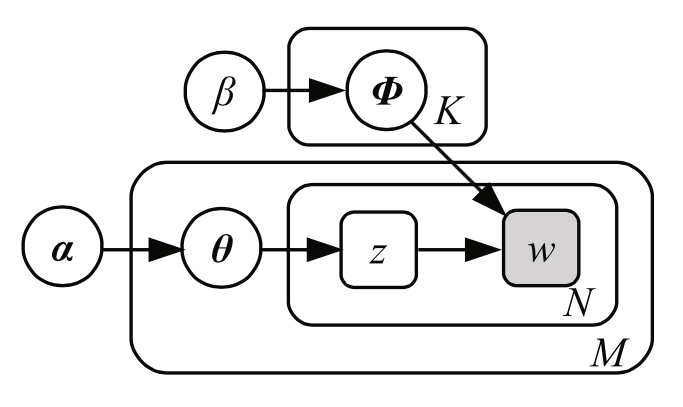
\includegraphics[width=0.8\textwidth]{lda.png}
\caption{LDA主题模型的概率图表示方式}
\label{fig:lda}
\end{figure}

如图\ref{fig:lda}所示,对于$M$篇文档、$K$个主题的语料库,文档-主题的分布为$\vec{\theta_m}~~(1\le m\le M)$,主题-词汇的分布为$\vec{\phi_k}~~(1\le k\le K)$。这两个随机变量与上文的词汇表类似,且都服从Dirichlet分布,即:
\begin{eqnarray}
  p(\vec{\theta}|\vec{\alpha})=Dir(\vec{\theta}|\vec{\alpha})=\frac{1}{\Delta(\vec{\alpha})}\prod_{i=1}^{K}\theta_{i}^{\alpha_i-1} \\
  p(\vec{\phi}|\vec{\beta})=Dir(\vec{\phi}|\vec{\beta})=\frac{1}{\Delta(\vec{\beta})}\prod_{i=1}^{W}\theta_{i}^{\beta_i-1}
\end{eqnarray}

在文档$d$中生成第$n$个单词的时候,首先要从文档-主题分布$\vec{\theta}$中抽样得到的主题编号为$z_{d,n}$,然后选取编号为$z_{d,n}$的主题-词汇分布$\vec{\phi}$,并抽样得到的一个单词$w_{d,n}$。由上面的理论可知,从Dirichlet分布抽样可以得到的观测值服从多项分布,记$\vec{x_d}=(x_{d,1},...,x_{d,K})$,$x_{d,k}~~(1\le k\le K)$表示在文档$d$中,抽样得到的编号为$k$的主题数量;同理,$\vec{y_d}=(y_{d,1},...,y_{d,W})$,$y_{d,v}~~(1\le v\le W)$表示在文档$d$中,抽样得到的词汇$v$的数量。$\vec{y_d}$和$\vec{y_d}$均为多项分布,即:
\begin{eqnarray}
  &&p(\vec{x_d}|\vec{\theta_d})=mult(\vec{x_d}|\vec{\theta_d})=
  \begin{pmatrix}
    N \\ \vec{x_d}
  \end{pmatrix}
  \prod_{i=1}^{K}\theta_i^{x_{d,i}} \\
  &&p(\vec{y_d}|\vec{x_d},\vec{\phi_d})=mult(\vec{y_d}|\vec{x_d},\vec{\phi_d})=
  \begin{pmatrix}
    N \\ \vec{y_d}
  \end{pmatrix}
  \prod_{i=1}^{W}\phi_i^{y_{d,i}}
\end{eqnarray}

有了以上基础之后,最终可以得到文档$d_m=\vec{w_m}$的生成概率为\cite{heinrich2005parameter}:
\begin{equation}
  p(d_m|\vec{\alpha},\vec{\beta})=\iint p(\vec{\theta_m}|\vec{\alpha})p(\Phi|\vec{\beta})\cdot \prod_{n=1}^{N_m}p(w_{m,n}|\vec{\theta_m},\Phi)d\Phi d\vec{\theta_m}
\end{equation}
所以整个语料库生成的概率为:
\begin{equation}
  p(\mathcal{D}|\vec{\alpha},\vec{\beta})=\prod_{m=1}^{M}p(d_m|\vec{\alpha},\vec{\beta})
\end{equation}

现在的问题转换成估计参数$\Theta=\{\vec{\theta_1},...,\vec{\theta_M}\}$和$\Phi=\{\vec{\phi_1},...,\vec{\phi_K}\}$。考虑到该问题涉及过多纯统计学知识,下文将直接使用成熟的collapsed Gibbs Sampling算法\cite{griffiths2004finding}进行求解,具体公式将不再列出。

\subsection{用户兴趣表示与匹配}
随着互联网上新型的网站越来越多,用户也会被各种各样的信息资源所吸引,而这些资源的主题可以在一定程度上反映出用户的兴趣所在。因此,将利用之前提出的文本信息分析与匹配方法先挖掘出隐藏在文本背后的主题,然后,通过发现并结合互联网用户兴趣的特点,提出一种可以全面且有效的表示方法和其对应的匹配机制。

首先,目前最常用的表示用户兴趣的方式是VSM,假设一共存在$K$种兴趣,并且兴趣之间没有关联性,而用户的兴趣则表示为一个$K$维向量$\vec{in}=(w_1,w_2,...,w_K),~~w_i\in [0,1](1\le i\le K)$,$w_i$表示用户对第$i$个兴趣的喜好程度。用VSM来表示用户兴趣的好处是在计算兴趣相似度的时候速度十分快,一般使用余弦相似度就能计算得出两个向量之间的距离。当余弦值越小就表示用户之间拥有更为相似的兴趣爱好。虽然这个方法在大部分情况下都十分快捷有效,但是,考虑到互联网用户的特点,上述方法存在下面两个问题,因此不能用于完全表示用户兴趣。
\begin{itemize}
  \item 兴趣关联性:由于用户的兴趣对应于文本资源中的主题,而主题之间是由相关性的,这种相关性体现在两个方面。一是主题之间的同义或反义,比如,CBA和NBA是两个主题,但是它们之间的共同点是都是篮球比赛,区别在于举办地点不同、规则不同等等。二是主题之间有层级关系,比如篮球和NBA是两个主题,篮球是一个更加广阔的概念,包括了篮球比赛、篮球运动员、实体篮球等,而NBA则是一个相对狭窄的概念,所以NBA这个主题是属于篮球的。
  \item 兴趣动态性:用户的兴趣一般可以分为长期兴趣和短期兴趣。长期兴趣相对稳定,变化较少,构建模型时比较容易。但是短期兴趣是一个难点,因为它会随着时间的变化而变化,而且每次持续的时间也都未知,可以近似把兴趣与时间的关系看成一个随机过程。
\end{itemize}

为了解决上述两个问题,第三章提出了一套完整的用户兴趣构建方式,包括一种叫做动态兴趣树的兴趣表示方式和一种层级结构的兴趣相似度衡量算法。动态兴趣树的表示方式解决了兴趣随着时间变化的问题,树中的每个节点表示一种兴趣,当用户兴趣发生变化时,这些节点存储的兴趣会通过旋转方式分辨出长期兴趣和短期兴趣。而层级结构的兴趣相似度算法是在主题模型的基础上,增加了层次结构,使得主题之间具有相关性。为了在第四章中更加简单和清晰地阐述这两种方法的构建和维护,这里先对用户兴趣模型的基本概念进行说明。

假设总共有$K$种兴趣点构成了兴趣全集$\mathcal{I}$,即$\mathcal{I}=\{in_1,in_2,...,in_K\}$,并且事先定义大小为$|V|$的词汇表$V$。对于兴趣点$in_k~~(1\le k\le K)$,是一个关于词汇的向量$in_k=(w_1,w_2,...,w_V)$,其中,$w_i~~(1\le i\le |V|)$表示词汇$v_i$在当前兴趣点$in_k$的重要程度。那么,兴趣点之间的相似度计算可以利用余弦相似度来计算两个向量的夹角。

\begin{figure}
\centering
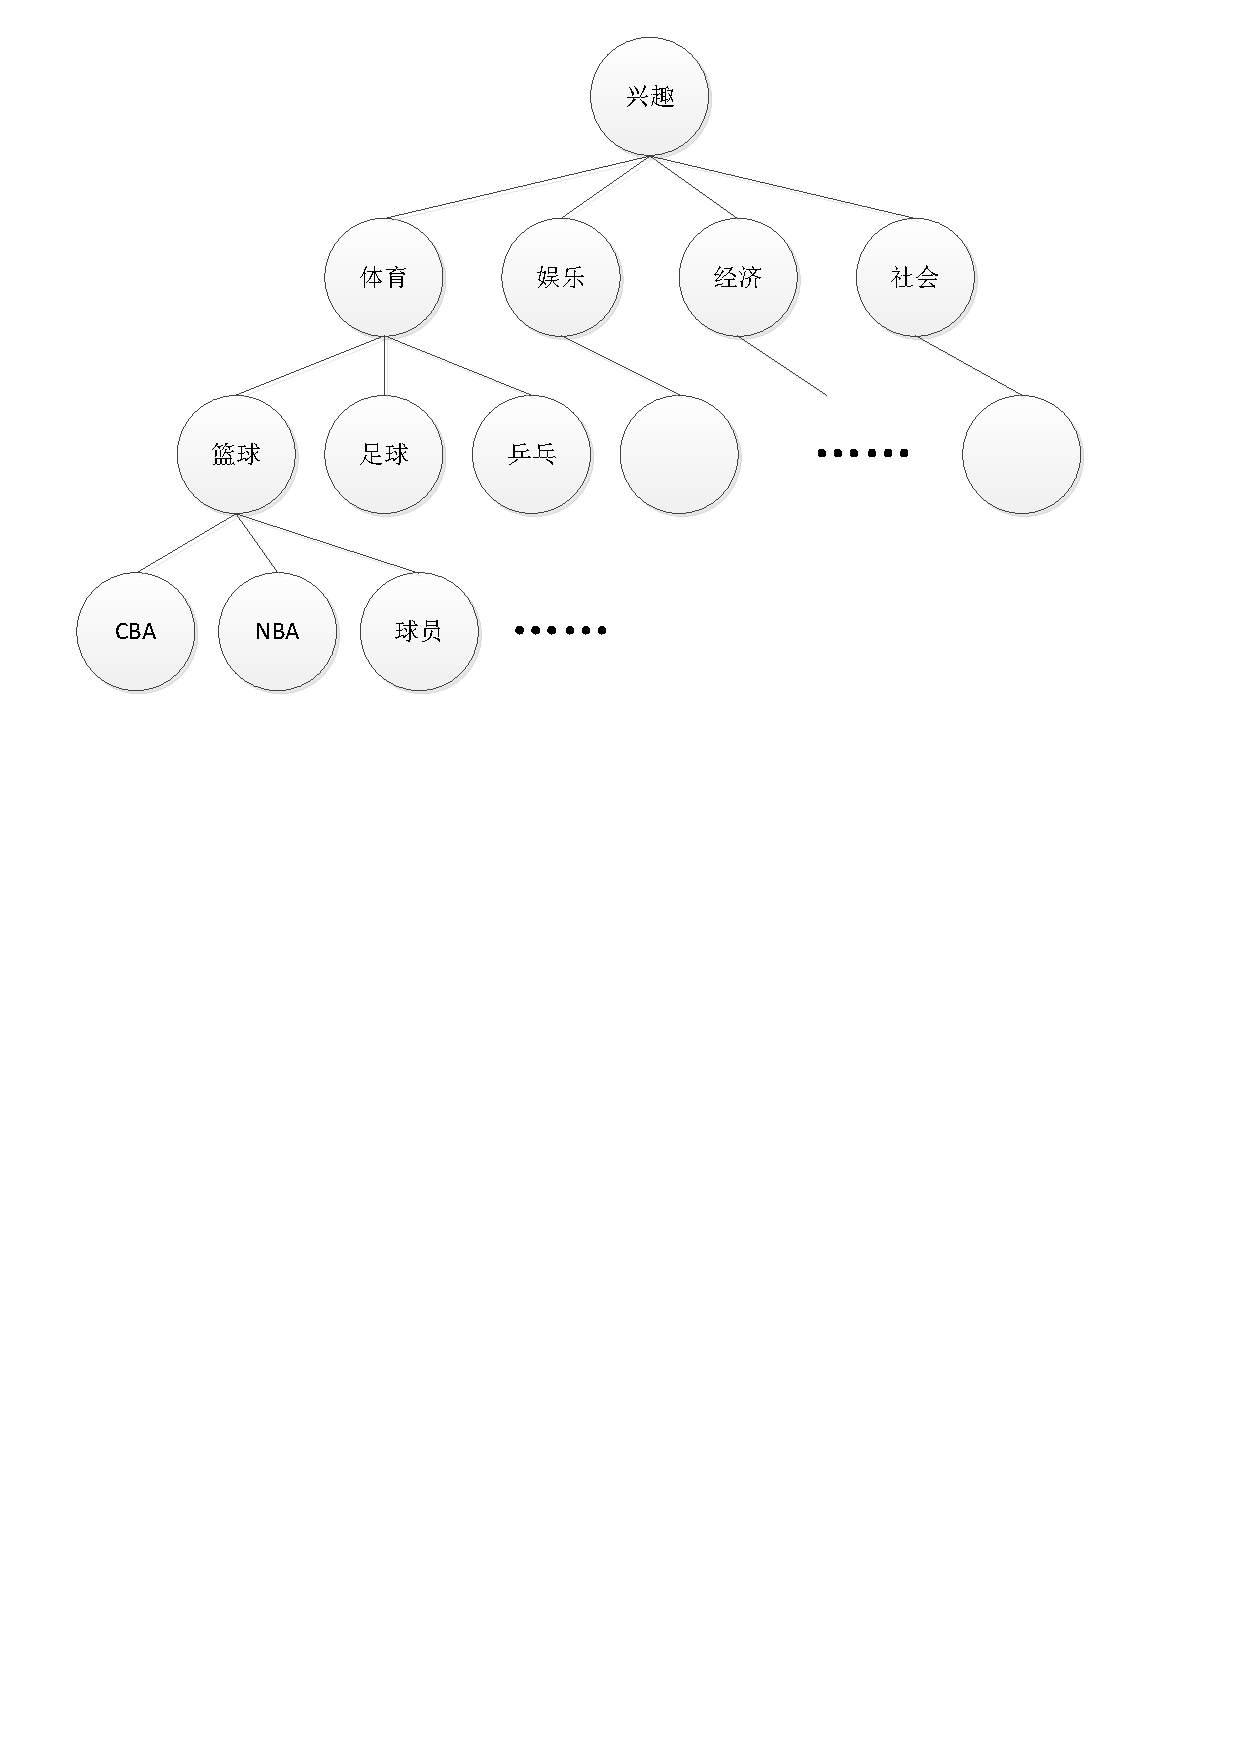
\includegraphics[width=0.8\textwidth]{interesttree.pdf}
\caption{静态兴趣分类树实例}
\label{fig:interesttree}
\end{figure}

普通的静态兴趣树是一种将兴趣点进行层次分类的表示方式,这种数据结构能够很好地表示出兴趣点之间的关联性。如图\ref{interesttree}所示,这是一棵四层结构的兴趣树,树上的每个节点表示一种兴趣点,距离根节点越近的节点表示范围越广泛。换句话说,在兴趣树上,父节点表达的兴趣点一般包含了其孩子节点所表达的内容,同时,处于同一层且拥有相同父节点的孩子节点一般具有部分交集的内容。于是,可以对兴趣全集$\mathcal{I}$中所有的兴趣点来构建一个完整的兴趣树。具体的构建方法可以分为人工构建法、半自动构件法和自动构建法。人工构建法可以借助词典来进行,因为在词典中定义了部分词汇的上义词、下义词、同义词,如果兴趣点$in$的名称正好在这部分词汇内,那么可以直接建立关系,然后再将剩余节点根据人为的经验来判断具体的位置。可以看到这种方法的精确性应该是最高的,因为它十分符合人正常的思维习惯,但是问题也十分明显,即当兴趣全集的数量十分巨大的时候,人工就十分费时费力了。因此,与人工构建法相对的是自动构建法,这种方法基于兴趣点相似度的计算方式,最简单的方法是计算余弦相似度。给定两个兴趣点$in_i$和$in_j$,余弦相似度$sim(in_i,in_j)$为:
\begin{equation}
  sim(in_i,in_j)=cos(in_i,in_j)=\frac{\sum_{k=1}^{|V|}w_{i,k}w_{j,k}}{\sqrt{\sum_{k=1}^{|V|}w_{i,k}^{2}\cdot\sum_{k=1}^{|V|}w_{j,k}^{2}}}
\end{equation}
然后,当构建第二层时(因为第一层的根节点不是兴趣点),对于给定的分类数量$N$,对所有兴趣点进行聚类,可以用常见的K-means算法进行计算。对于每一个类中,对每个兴趣点进行两两的相似度计算,从而得到一个兴趣点之间的相关性矩阵$A$:
\begin{equation*}
  A=\left(
  \begin{array}{cccc}
    a_{1,1} & \cdots & a_{1,j} & \cdots \\
    \vdots & \ddots & \vdots & \\
    a_{i,1} & \cdots & a_{i,j} & \cdots \\
    \vdots & & \vdots & \ddots \\ 
  \end{array}
  \right)
\end{equation*}
其中,$a_{i,j}=sim(in_i,in_j)$。接着,对矩阵$A$中的每个行向量计算均值$mean(\vec{a_i})$和方差$var(\vec{a_i})$,选择均值较大方差较小的行向量,其对应的兴趣点作为第二层的一个节点。依次类推完成其他节点的构建。可以发现,自动构建法适用于大规模兴趣点的场景,但是精确度比人工构建法会差一点,因此,一般使用半自动构建法,即结合人工反馈的方式和自动分类的方式进行构建,具体方法将在第四章中详细说明。同时,对于每个用户$u$来说,其各自还需要维护一棵兴趣子树,从而可以进行用户之间两两的兴趣匹配。

此外,这种静态的分类兴趣树仅仅描述了兴趣点之间的关联性,但是用户的兴趣还分为长期兴趣和短期兴趣,对于动态变化的短期兴趣来说,这种静态的结构不太适合,因此提出了一种基于二叉伸展树结构的动态兴趣树,r其基本原理是每当用户有新的兴趣加入时,将交换已有树中的节点位置,离根节点越近的节点说明是用户最新的兴趣,相反离得越远的节点说明用户只是在很久以前曾经有过的兴趣。如图\ref{fig:splaytree}所示,当系统发现最近用户对季后赛有了浓厚的兴趣时,伸展树的结构就会发生变化,季后赛节点从左边旋转到根节点,表示用户当前最感兴趣的一项。

\begin{figure}
\centering
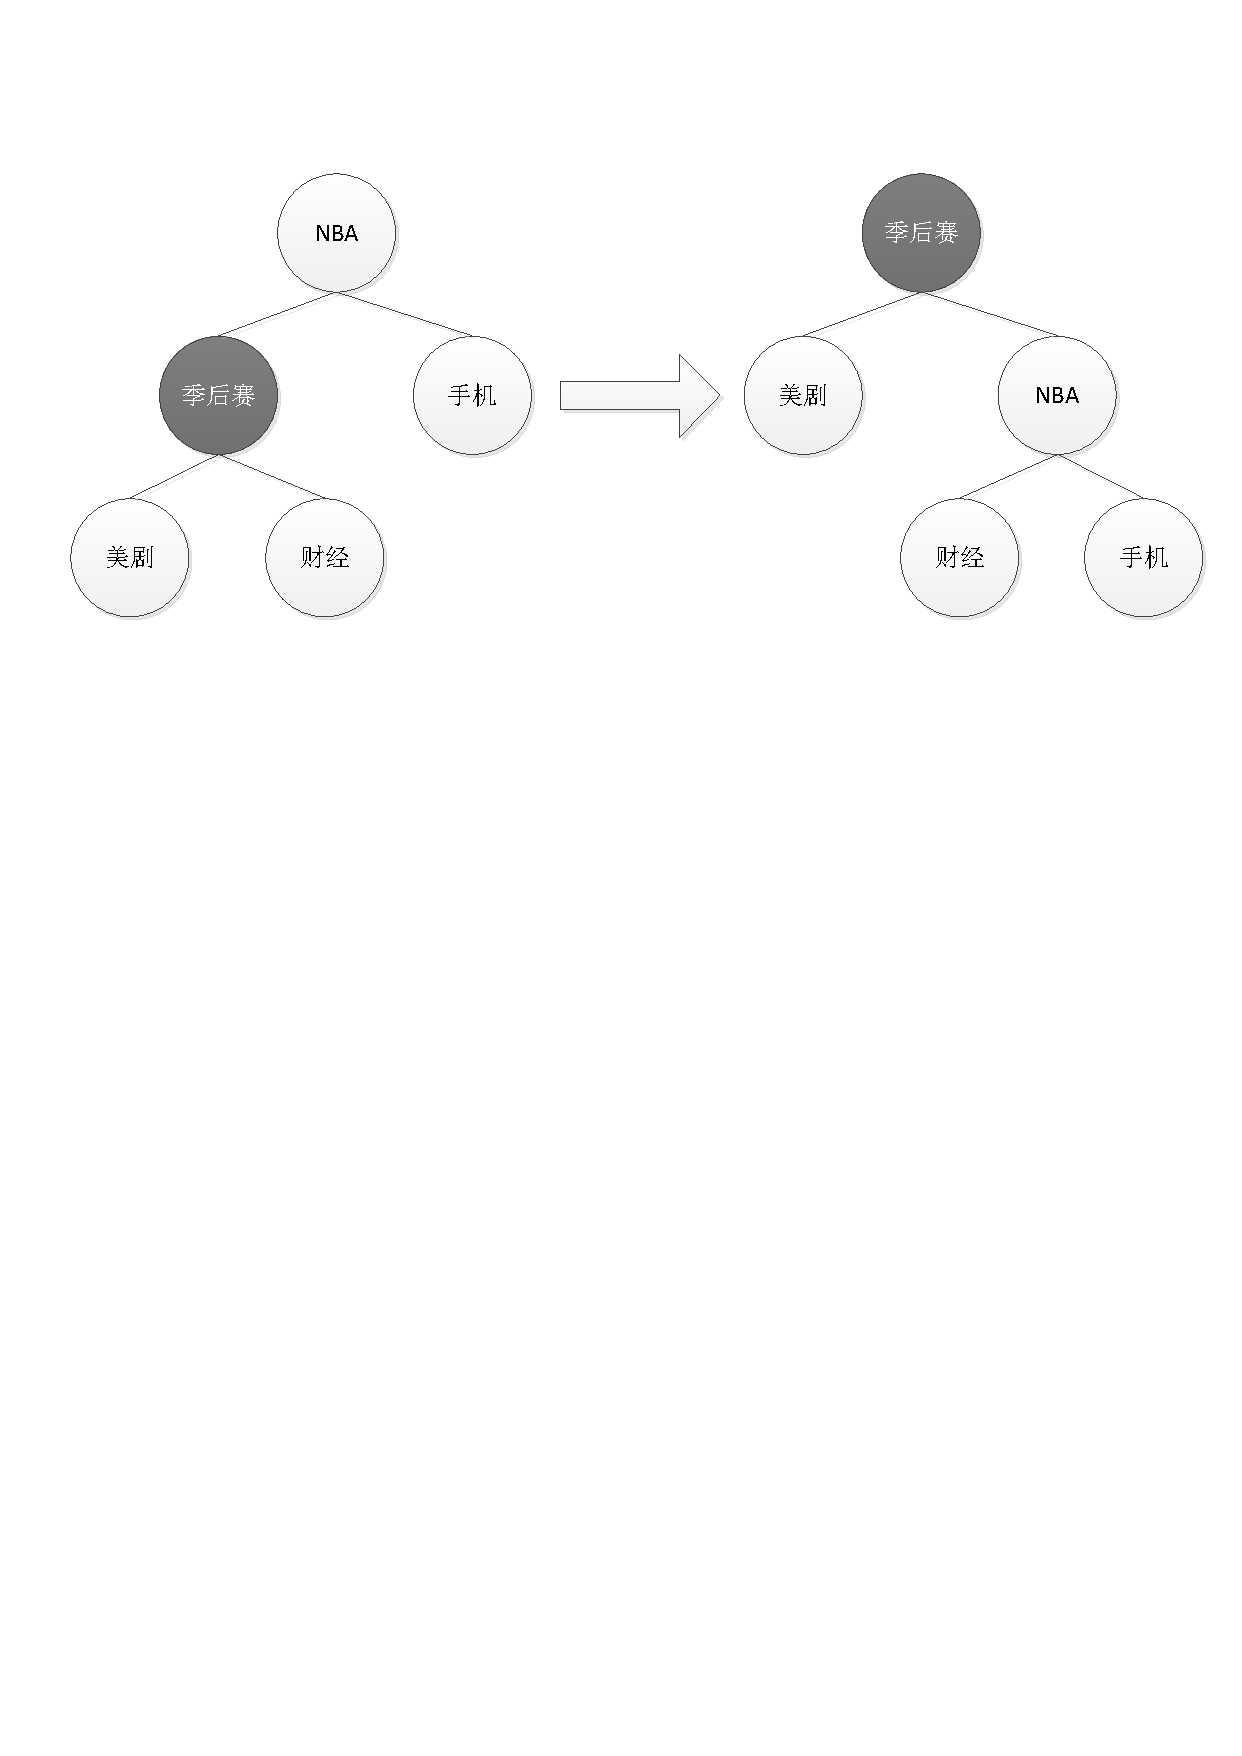
\includegraphics[width=\textwidth]{splaytree.pdf}
\caption{动态兴趣伸展树实例}
\label{fig:splaytree}
\end{figure}

二叉伸展树是一种自适应的二叉搜索树,其遵循的特点是近期访问过的节点将会在不久之后又被访问到。对于诸如插入节点、查找节点、和删除节点等基本操作都在$O(log~n)$的时间内。对于一系列非随机的操作,伸展树的性能比其他搜索树表现得更好。这一点尤为重要,因为在互联网中,用户的兴趣变更十分频繁,这些变更的操作包括了加入新的兴趣、重新对已有兴趣有了热情等等,之所以选择二叉伸展树就是因为其可以表现出这个特征。另外,伸展树的性能在一定程度上取决于它的自优化过程,频繁操作的节点比不操作的节点更容易接近根节点。伸展树的高度在最坏情况达到了$O(n)$,但平均情况稳定在$O(log~n)$,最坏情况下伸展树的高度成为了最主要的弊端。

但是,在兴趣伸展树中不能体现出兴趣点之间的联系,因此需要将静态和动态的兴趣树结合起来判断用户的完整兴趣,具体方法将在第四章中详细说明。

\subsection{P2P网络构建与发现}
基于上述两部分的工作,接下来要在已有的网络架构上建立一层P2P网络来实现信息自主流动的机制。在构建网络之前,必须确保理解以下几个关于信息流动的问题。
\begin{itemize}
  \item 信息流动的目的:互联网上的信息内容众多,但是用户真正需要的信息不多,因此信息流动的本质是为了让用户获得更多有用的信息,过滤掉相对没用的信息。这个过程与信息推荐有所类似,但是也有所不同,相同点是用户都是被动地接受处理过后的信息,但不同点是,现在推荐系统都是基于集中式的架构,而此处信息流动是一个更加广域的概念,其基础是建立在P2P的网络中。
  \item 信息流动的依据:在文本中,用户有用的信息是指用户真正感兴趣的内容,用户兴趣模型的作用就是先挖掘出用户的潜在兴趣,然后匹配信息的主题与用户兴趣之间的关联度,并进行推荐。换句话说,信息流动是由用户兴趣所驱动的,因此只要衡量目标用户的兴趣与信息发布者的资源是否相似即可。
\end{itemize}

因此,要建立的P2P网络是建立在用户兴趣的基础之上的,或者更确切的说法是,将在已有的网络架构上添加一层基于P2P架构的用户兴趣覆盖网络,从而使得信息能够在这一层网络中进行自动传播。为了说明兴趣覆盖网络的基本概念,本节用暂时使用VSM模型来表示用户兴趣。

首先,在基于P2P架构的兴趣覆盖网络上,先有一层用户好友关系层。其中,每个用户表示一个节点,用户集合$U$可以表示为:
\begin{equation*}
  U=\{u_1,u_2,...,u_{|U|}\}
\end{equation*}
$|U|$表示用户集合的大小。

在目前传统的网络中,用户之间可以相互加为好友,把这种好友的关系定义为follower和followee的单向关注的关系:
\begin{equation*}
  \forall u_i,u_j \in U, \exists e_{i,j}:~u_i \to u_j
\end{equation*}
如果用户$u_i$关注了用户$u_j$,$u_i$和$u_j$之间则存在一条边$e_{i,j}$。那么所有的关注关系集合$E_f$可以表示为:
\begin{equation*}
  E_f=\{e_{i,j}|u_i\to u_j,1\le i,j\le n\}
\end{equation*}
于是用户集合和关系集合构成一张有向图$G_f=\{U,E_f\}$。

接下来,要在用户好友关系层上加上兴趣覆盖网络。假设兴趣全集定义与上面相同,即表示为:
\begin{equation*}
  \mathcal{I}=\{in_1,in_2,...,in_{|\mathcal{I}|}\}
\end{equation*}

用户$u$的兴趣可以用向量简单地表示为:
\begin{equation*}
  d_u=(w_{u,1},w_{u,2},...,w_{u,|\mathcal{I}|})
\end{equation*}
其中$w_{u,i}\in [0,1]~~(1\le i\le |\mathcal{I}|)$表示用户$u$对兴趣点$in_i$实际感兴趣的程度。对于给定的阈值$\epsilon$,当且仅当$w_i>\epsilon$时,称用户$u$拥有兴趣点$in_i$,否则用户$u$不拥有兴趣点$in_i$。

对于两个用户$u_i$和$u_j$,他们的兴趣向量分别是$d_{u_i}$和$d_{u_j}$,如果存在$k~(1\le k\le |\mathcal{I}|)$,满足条件:
\begin{equation*}
  w_{u_i,k}>\epsilon~~\mbox{并且}~~w_{u_j,k}>\epsilon
\end{equation*}
那么称用户$u_i$和用户$u_j$分享共同的兴趣点$in_k$。于是在兴趣覆盖网络中,这两个节点之间存在一条边$v_{i,j}^k:u_i\xleftrightarrow{k} u_j$。兴趣关系集$V_i$则表示为:
\begin{equation*}
  V_i=\{v_{i,j}^{k}|u_i\xleftrightarrow{k} u_j,1\le i,j\le n\}
\end{equation*}
用户集合与兴趣关系集合组成了兴趣覆盖网络$G_i=\{U,V_i\}$。

\begin{figure}
\centering
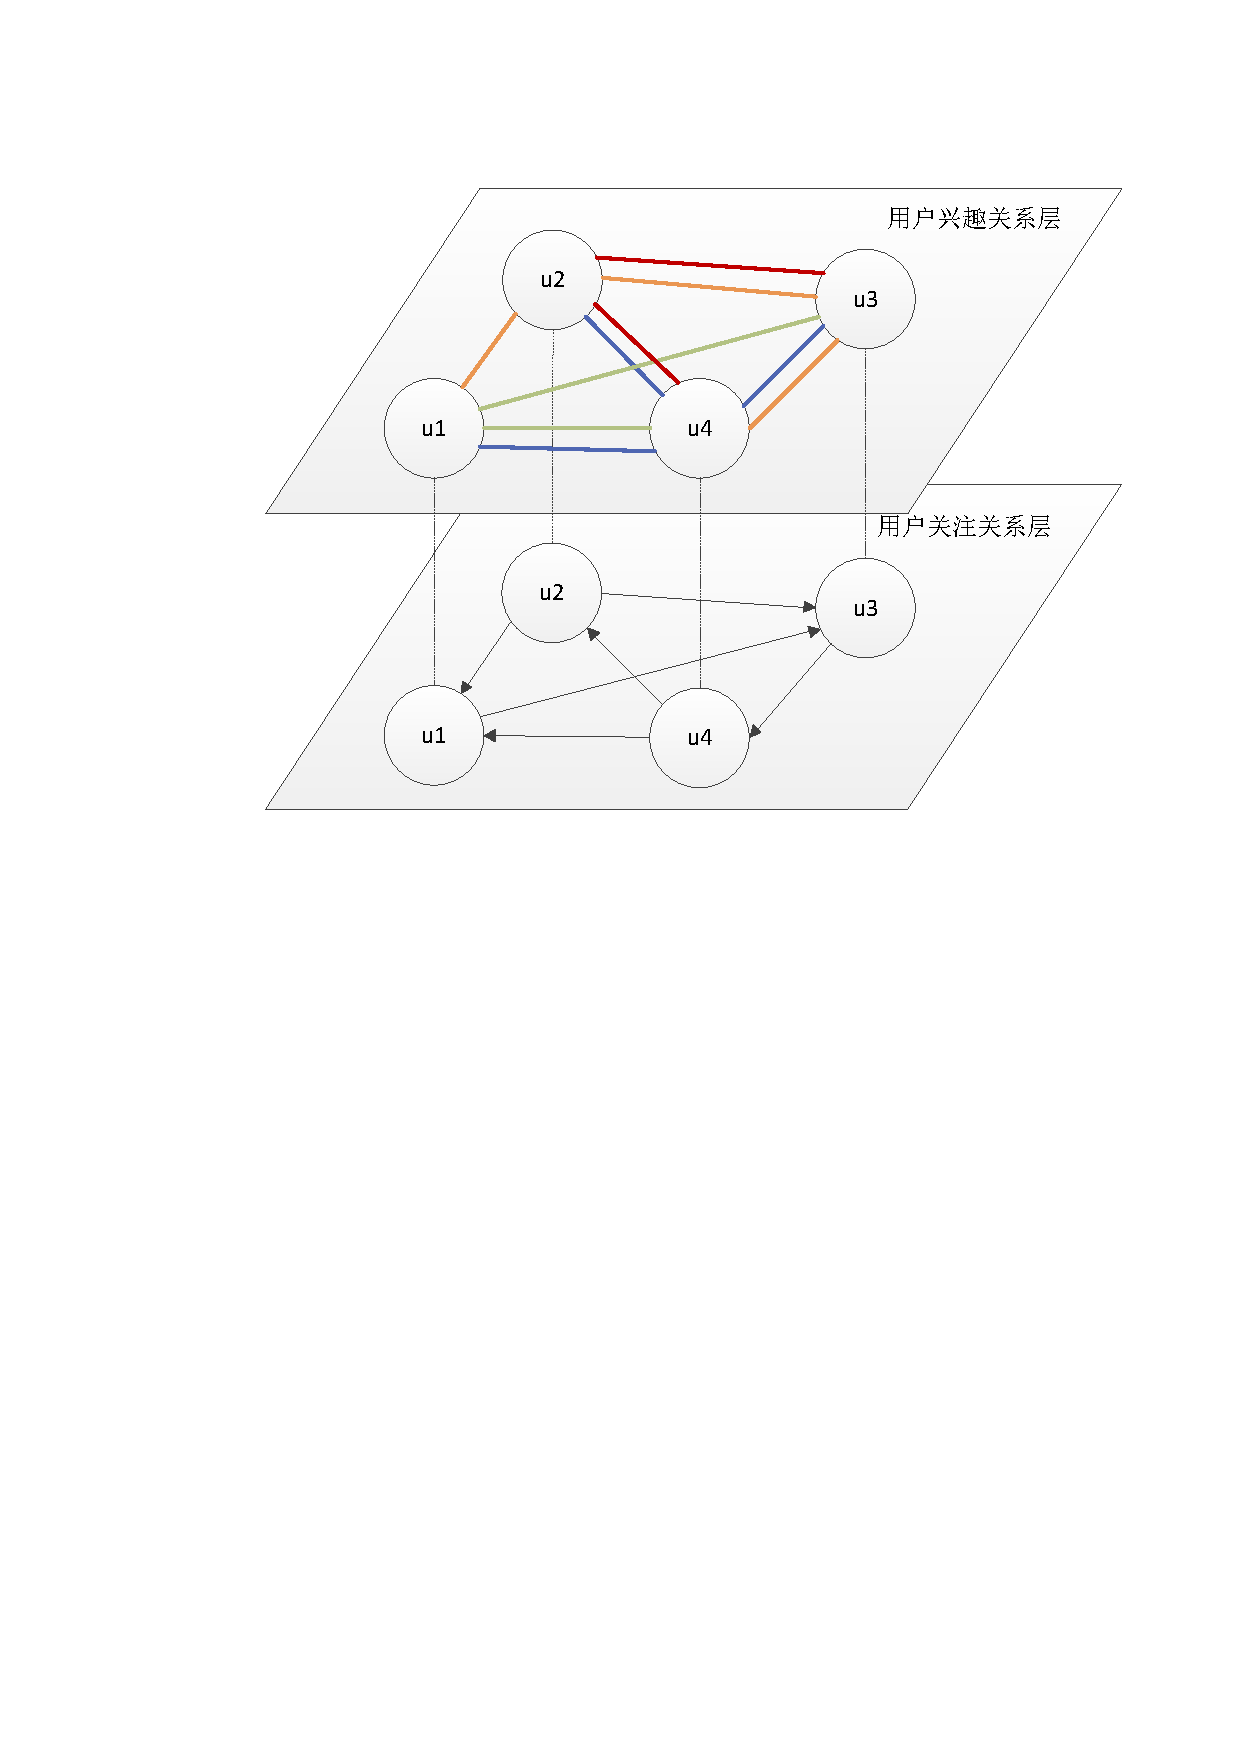
\includegraphics[width=\textwidth]{interestlay.pdf}
\caption{基于向量表示的兴趣覆盖网络实例}
\label{fig:interestlay}
\end{figure}

如图\ref{fig:interestlay}所示,在一个简化的四节点的网络结构中,可以看到在用户关注关系层上,$u_1,u_2,u_3,u_4$四个用户之间存在着单向的关注关系,但是在这一层上不能直观地看到用户之间存在哪种相关性,这导致了在路由搜索的时候性能下降(在搜索过程中再进行匹配会很慢)。所以,在用户关注关系层上添加了一层用户兴趣关系层,在这一层中,四个用户相对位置并没变化,但是他们之间多出了几条彩色的边,即共同兴趣关系边,这里不同的颜色表示不同的兴趣点。两个用户之间可以存在一条或多条兴趣边,因为他们之间可能存在的共同兴趣不止一个。当然,在这一层中,节点之间存在多条边的关系不能在后续的搜索过程中进行路由,甚至会造成多重环的问题。所以,在计算过程中,可以将两节点间多条边转换成一条权重为向量的边,具体计算方式会在第五章中详细阐述。

\subsection{小结}
在这一章中, 简单阐述了基于P2P网络的信息自主流动机制的方案,在这一机制中主要涉及三大模块:文本信息的分析与建模、用户兴趣的表示与匹配和P2P网络的构建与发现。其中,在文本信息分析与建模的问题中,分析了直接用VSM模型来描述互联网资源的弊端,并且根据问题的根结所在,提出了用主题来表示资源是一个更好的方法。一方面对文本的高维度进行了降维,另一方面也表达出了文本隐藏在背后的含义。然后,通过模拟文本的生成过程,从而解释了对文本主题求解的基本方案。在用户兴趣表示与匹配的问题中,首先基于兴趣之间的相关性和兴趣动态变化两大特点,分别提出了两种解决方案:静态兴趣分类树和动态兴趣伸展树。在P2P网络的构建与发现问题中,引入了兴趣覆盖网络这一概念,并且用简单的基于VSM的兴趣模型来说明兴趣覆盖网络的直观意义和表示方法。
